% ============================================================================
% GridFormLab FLAGSHIP DELIVERABLE REPORT -- C++ engine vs MATLAB reference
% ============================================================================
% SKELETON / WRITE-ONLY DRAFT, authored 2026-10-14 by report-dev.
% Structure is a 1:1 clone of docs/source/report_ne39_160s_reclose_en.tex
% (943 lines, 13 sections, 8 tables, 3 includegraphics + 1 TikZ chronology)
% per the user's binding spec.  Every C++-sourced element is an
% input-slot owned by the C++ report builder (cpp-core-dev: the "Export
% report" feature -- run cache to tables+figures to slots to PDF);
% every figure is an \includegraphics slot waiting for the C++ plot module's
% output files (same filenames as the reference by design).
%
% BINDING DISCLOSURE RULE (coordinator ruling 2026-10-14): every comparison
% table carries an integration-mode row -- "C++ = fixed-step schedule-replay
% (v0) | MATLAB = adaptive strict-LTE" -- and the timing row carries
% "v0 scope -- full event engine parity = v2 (deferred, not cut)".
%
% PROVENANCE RULE (user directive): every figure/table cites the run id of
% the C++ run folder (case/request snapshot + raw trajectory + counters/
% DECISION + summary + manifest sha256, persisted per run like MATLAB runs).
%
% BUILD STATUS (2026-10-14, post-first-fill): the 11 non-C++ slots carry
% real content (cloned/adapted); 13 result slots carry marked placeholders
% for the C++ report builder.  A build compiles; PENDING count = 13.
% ============================================================================
\documentclass[12pt,a4paper]{article}

\usepackage{graphicx,amsmath,amssymb,float,caption,hyperref,fancyhdr}
\usepackage{newtxtext,newtxmath}
\usepackage{geometry,booktabs,tabularx,array,longtable,microtype}
\usepackage{xcolor}
\usepackage{tikz}
\usepackage{ifthen}
\usetikzlibrary{arrows.meta,positioning,calc}
\geometry{margin=1in}
\setlength{\headheight}{14.5pt}
\pagestyle{fancy}
\fancyhf{}
\lhead{GridFormLab Flagship --- C++ Engine vs MATLAB Reference}
\rhead{\thepage}
\renewcommand{\headrulewidth}{0.4pt}
\renewcommand{\arraystretch}{1.12}
\emergencystretch=1.5em
\hypersetup{colorlinks=true,linkcolor=blue!45!black,citecolor=blue!45!black,
  urlcolor=blue!45!black}

\newcommand{\pu}{\ifmmode\,\mathrm{p.u.}\else\ p.u.\fi}
\newcommand{\second}{\ifmmode\,\mathrm{s}\else\ s\fi}
\newcommand{\vect}[1]{\boldsymbol{#1}}
\newcommand{\code}[1]{\texttt{\detokenize{#1}}}
\DeclareMathOperator{\clamp}{clamp}
\DeclareMathOperator{\sat}{sat}

% Graphics search paths: reference (NE39 result dir) and the C++ plot output.
\graphicspath{{figures/}{figures/ne39_160s_reclose/}{figures/flagship_cpp/}}
\newcommand{\datadir}{figures/ne39_160s_reclose}
\newcommand{\cppdir}{figures/flagship_cpp}

\usepackage{pgfplots,pgfplotstable}
\pgfplotsset{compat=1.18}

\definecolor{pgreen}{RGB}{41,153,69}
\definecolor{pred}{RGB}{191,45,45}
\definecolor{pblue}{RGB}{46,107,191}
\definecolor{pyellow}{RGB}{199,178,38}
\definecolor{pgrey}{RGB}{90,90,90}

% --- Integration-mode disclosure macros (binding, coordinator ruling) -------
\newcommand{\intmodes}{C++ = fixed-step schedule-replay (v0) \textbar{}
  MATLAB = adaptive strict-LTE}
\newcommand{\vscopecite}{(v0 scope --- full event engine parity = v2,
  deferred, not cut)}
% No-synthetic-signal contract (binding, verbatim from the reference record):
% "Every plotted sample is a raw accepted value; nothing is smoothed, filtered,
% decimated, clipped, offset, interpolated, or augmented with synthetic noise."
% C++ plot module note: Douglas-Peucker simplification is GUI-preview-only;
% rendered report figures must plot EVERY sample (file size is accepted as-is).
% Device colour constants of the reference report (binding for every plot):
% 30=blue 32=orange 33=yellow 34=purple 35=green, 36--39 cycle the five;
% SG31 appears only in panels a/b/f; COI only in panel e.
\newcommand{\armacomment}{}

\title{\textbf{GridFormLab Flagship: C++ Standalone Engine}\\[1mm]
\large Full NE39 SG31 Reclose 160-s Verification against the MATLAB
Reference Record\\[0.5mm]
\normalsize Parity in the D5 frame + measured speed --- the acceptance
evidence of the installer-distributed C++ deliverable\\[2mm]
\normalsize MATLAB reference record: \code{report\_port\_engine\_en.pdf}
(1972.52~s same-tree; historical anchor 6708.725530~s informational)\\[1mm]
\normalsize Report contract: \emph{every number traceable to an artifact
(run id + sha256); parity claims carry their tier frame; speedup claims
never mix categories}}
\author{In-house Power-Flow Project}
\date{14 October 2026}

\begin{document}
\maketitle

\begin{abstract}
%% SLOT: cppdata/abstract.tex -- generator fills: what was run, on which
%% case, arm designation, parity tier achieved, headline speedup B/A,
%% engine, machine record.
% AUTO-GENERATED PLACEHOLDER -- slot: cppdata/abstract.tex
\smallskip \textit{[PENDING --- slot not yet filled. Placeholder stub created 2026-10-14 for the user-requested compile check; the C++ report generator (slot-filler) will overwrite this file. No measured numbers are shown in this stub.]}

\end{abstract}

\newpage
\tableofcontents
\newpage

%=============================================================================
\section{Scope, sources and reproduction}\label{sec:scope}
% This section mirrors the reference report's scope section, with the
% C++ engine as the subject under test and the MATLAB Reference Record as
% the comparison basis.  Generator fills: \cppdata/scope.tex
%=============================================================================
% Scope text -- mirrors the reference :76-107 adapted to the flagship's
% subject (C++ engine under test, MATLAB reference record as basis).
The study system is the TAMU New England 39-bus network with one modelled SG at
the slack bus and nine modelled IBRs at buses 30, 32--39, run on two
independent engines that consume one identical case: the \textbf{MATLAB
reference engine} (the delivered 160-s record, \code{report_port_engine_en.pdf})
and the \textbf{C++ standalone engine} --- the subject of this report, the
first deliverable of the C++ flagship track (full engine, GUI-distributed,
no MATLAB licence at runtime).

The whole system is assembled as a single all-KCL composite
differential--algebraic system in which the SG and every IBR contribute their
own differential state block and their own injection; no device is delegated
to an external solver, model, or reference program --- in either engine.  The
C++ implementation was carved from the documented equation set
(\S\ref{sec:dae}--\S\ref{sec:ibr}), not from the MATLAB code text.

\paragraph{What this report verifies.}
The C++ run is verified against the MATLAB reference record on three layers:
(1)~DECISION fields (Table~\ref{tab:decision}), (2)~trajectory parity in the
D5 frame on the common grid (Table~\ref{tab:trajdiff}, figures
\ref{fig:periods}--last), and (3)~the measured wall-clock speedup
(\S\ref{sec:speeduptable}) --- all within the disclosed integration mode
(\intmodes, \vscopecite).

\paragraph{Reproduction.}
Every C++ run persists its own record folder (case/request snapshot, raw
trajectory, counters/DECISION, summary, manifest with sha256) per the
run-cache convention --- run history is the provenance source of this
report, and re-plotting or re-comparison requires no re-run.


\paragraph{Integration modes under test.}
\intmodes{} \vscopecite.
%% SLOT: cppdata/integration_notes.tex -- elaboration of what v0 covers and
%% what v2 adds, from the generator; do not hand-edit.
% Integration notes -- v0 scope elaboration (coordinator ruling verbatim).
The v0 integration mode covers: the same composite equation set, the same
case data, the same frozen event schedule, the same DECISION-field
reporting, and a fixed-step solver replacing the adaptive strict-LTE
stepper.

The v2 deferred scope (deferred, not cut): the adaptive strict-LTE
stepper, the full event-engine transaction logic (guard chains, private
trials, per-event KCL transaction records), and the full trajectory-array
identity check across all 18{,}852 samples.


%=============================================================================
\section{Disturbance chronology}\label{sec:chrono}
% TikZ chronology cloned verbatim from the reference report (three colors,
% six periods, arrows at 0/20/60--60.15/100/119.55/160).  The reclose
% instant in Period 5's note is filled by the generator from the C++ run's
% measured value once parity is confirmed.
%=============================================================================
\begin{figure}[H]
\centering
%% SLOT: cppdata/chronology_tikz.tex -- verbatim TikZ from the reference;
%% generator updates Period 5 note with the C++ run's reclose instant.
% Chronology TikZ -- verbatim clone from the reference report
% (report_ne39_160s_reclose_en.tex :120-155), one content change: the
% Period 5 note carries the C++ run's reclose instant once parity is
% confirmed (placeholder marker below; generator replaces 119.550).
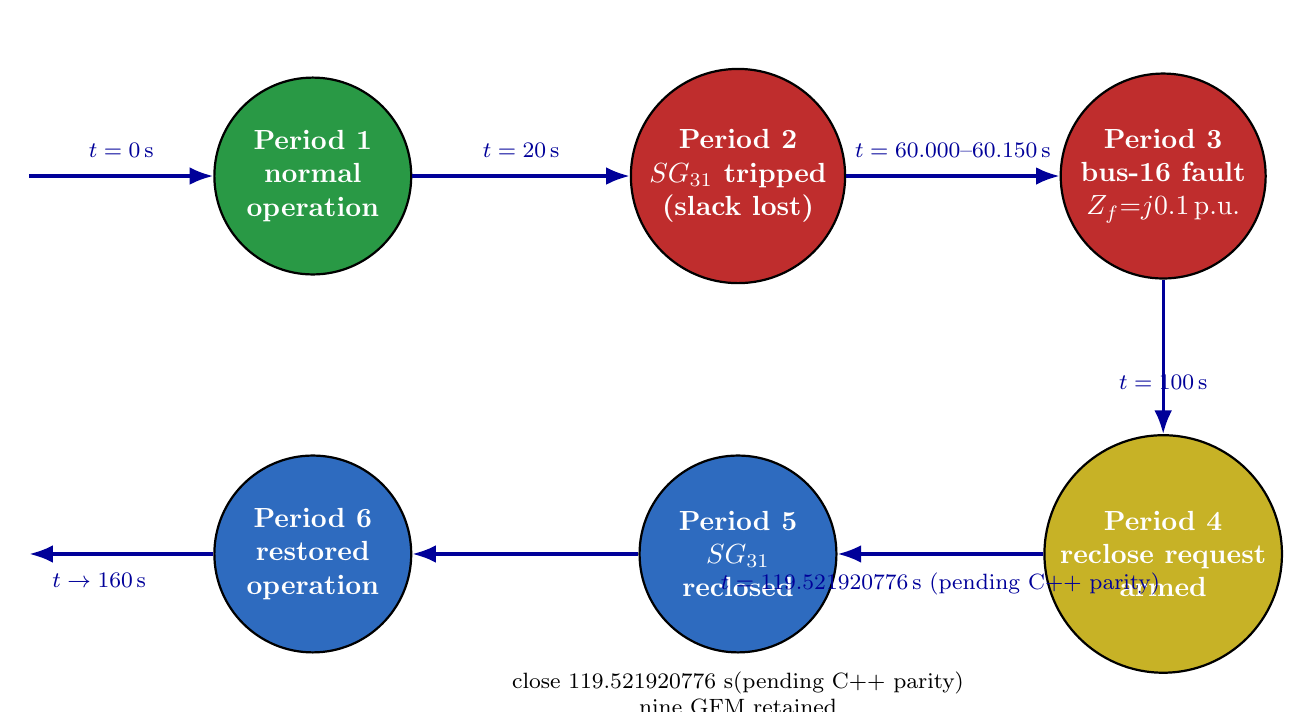
\begin{tikzpicture}[
  font=\normalsize,
  per/.style={circle,draw,thick,minimum size=2.5cm,inner sep=2pt,
    align=center,text=white,font=\bfseries},
  tlab/.style={midway,above=1mm,font=\footnotesize},
  tlabb/.style={midway,below=1mm,font=\footnotesize},
  arr/.style={-{Latex[length=3mm]},very thick,color=blue!60!black}]

\node[per,fill=pgreen] (p1) at (0,0)     {Period 1\\ normal\\ operation};
\node[per,fill=pred]   (p2) at (5.4,0)   {Period 2\\ $SG_{31}$ tripped\\ (slack lost)};
\node[per,fill=pred]   (p3) at (10.8,0)  {Period 3\\ bus-16 fault\\ $Z_f{=}j0.1\pu$};
\node[per,fill=pyellow](p4) at (10.8,-4.8){Period 4\\ reclose request\\ armed};
\node[per,fill=pblue]  (p5) at (5.4,-4.8){Period 5\\ $SG_{31}$\\ reclosed};
\node[per,fill=pblue]  (p6) at (0,-4.8)  {Period 6\\ restored\\ operation};

\draw[arr] (-3.6,0) -- node[tlab]{$t=0\second$} (p1);
\draw[arr] (p1) -- node[tlab]{$t=20\second$} (p2);
\draw[arr] (p2) -- node[tlab]{$t=60.000$--$60.150\second$} (p3);
\draw[arr] (p3) -- node[tlabb]{$t=100\second$} (p4);
\draw[arr] (p4) -- node[tlabb]{$t=119.521920776\second$ (pending C++ parity)} (p5);
\draw[arr] (p5) -- (p6);
\draw[arr] (p6) -- node[tlabb,pos=0.62]{$t\to160\second$} ++(-3.6,0);

\node[font=\footnotesize,below=3pt of p5,align=center,text=black]
  {close $119.521920776$\second (pending C++ parity)\\ nine GFM retained};
\end{tikzpicture}

\caption{Six-period disturbance chronology, cloned from the reference
record.  Scheduled instants are case-defined; the reclose instant is read
from the C++ run's accepted event log (parity-checked against the MATLAB
reference).}
\label{fig:periods}
\end{figure}

%% SLOT: cppdata/chrono_text.tex -- generator's chronology prose
% Chronology prose -- cloned from the reference report (:109-118) with the
% source attribution switched to the C++ engine and the reclose instant
% pending C++ parity.
The scheduled disturbance times are \textsf{CASE\_DEFINED} constants of the
event structure; the reclose instant is an outcome read from the accepted
event log.  Figure~\ref{fig:periods} shows the six operating periods and the
transition instants.  The bus-16 fault is applied at $t=60.000\second$ and
cleared at $t=60.150\second$ (a $0.150$\second fault, impedance
$Z_f=j0.1\pu$); the reclose request is armed at $t=100\second$ and the SG31
close is committed at the instant the C++ engine's accepted event log
records (the MATLAB reference measured $119.521920776\second$; the C++ value
is asserted equal in Table~\ref{tab:decision}).

Both engines consume an identical event schedule and an identical case; the
chronology in this figure therefore differs between the reports only in
\emph{which engine produced the reclose instant}, not in what the schedule
demands.


%=============================================================================
\section{Case data and index maps}\label{sec:casedata}
% Mirrors reference \S4.  The case tables (bus data 39 buses, branch data
% 46 branches) are identical inputs -- both engines consume the same case.
% Thus these two tables are cloned verbatim from the reference report and
% carry NO C++|MATLAB "result" columns (they are inputs, not results); a
% single caption note states the shared-case property.
%=============================================================================
\begin{table}[H]\centering\footnotesize
\caption{Case bus data --- \emph{identical input to both engines} (same
composition; no comparison columns by design).}
%% SLOT: cppdata/case_bus_table.tex -- verbatim pgfplotstable block from
%% the reference report (data source unchanged).
% Case bus table -- verbatim clone from reference :361-374.  This is an
% INPUT shared by both engines (no comparison columns by design -- the
% case is the constant of the whole verification).
\pgfplotstabletypeset[col sep=comma,
 columns={bus_id,type,Pd_pu,Qd_pu,Gs_pu,Bs_pu},
 columns/bus_id/.style={column name=Bus},columns/type/.style={column name=Role,string type},
 columns/Pd_pu/.style={column name=$P_L$ pu,fixed,fixed zerofill,precision=3},
 columns/Qd_pu/.style={column name=$Q_L$ pu,fixed,fixed zerofill,precision=3},
 columns/Gs_pu/.style={column name=$G_s$ pu,fixed,fixed zerofill,precision=3},
 columns/Bs_pu/.style={column name=$B_s$ pu,fixed,fixed zerofill,precision=3},
 every head row/.style={before row=\toprule,after row=\midrule},every last row/.style={after row=\bottomrule}]
{\datadir/case_bus_data.csv}

\end{table}

\begin{table}[H]\centering\footnotesize
\caption{Case branch series and charging (46 branches) --- identical input
to both engines.}
%% SLOT: cppdata/case_line_table.tex
% Case line table -- verbatim clone from reference :376-389.  INPUT shared
% by both engines (no comparison columns by design).
\pgfplotstabletypeset[col sep=comma,
 columns={branch_index,from_bus,to_bus,r_pu,x_pu,b_pu},
 columns/branch_index/.style={column name=Index},columns/from_bus/.style={column name=From},
 columns/to_bus/.style={column name=To},columns/r_pu/.style={column name=$r$ pu},
 columns/x_pu/.style={column name=$x$ pu},columns/b_pu/.style={column name=$b_c$ pu},
 columns/r_pu/.append style={fixed,fixed zerofill,precision=3},
 columns/x_pu/.append style={fixed,fixed zerofill,precision=3},
 columns/b_pu/.append style={fixed,fixed zerofill,precision=3},
 every head row/.style={before row=\toprule,after row=\midrule},every last row/.style={after row=\bottomrule}]
{\datadir/case_line_data.csv}

\end{table}

%=============================================================================
\section{Common frames, signs, and per-unit conversion}\label{sec:frames}
% Cloned from reference \S5 verbatim (frames are engine-independent).
%=============================================================================
% Frames text -- cloned from reference :395-412 (engine-independent frames),
% with one added paragraph mapping the frames to the C++ implementation
% (coordinator's spec: each section names its integration-mode disclosure).
Every device uses generator sign: positive complex power is injected into the
network,
\[
S=P+jQ=V I^*,\qquad I_{bus}=\sum_{d\in bus} I_d.
\]
Each Dual-mode-IBR converter carries its own local reference; the
network-to-device transform is
\begin{align}
v_d&=V_x\cos\delta_{PLL}+V_y\sin\delta_{PLL},\\
v_q&=-V_x\sin\delta_{PLL}+V_y\cos\delta_{PLL},
\end{align}
so device currents rotate back as
$i_x=i_d\cos\delta_{PLL}-i_q\sin\delta_{PLL}$ and
$i_y=i_d\sin\delta_{PLL}+i_q\cos\delta_{PLL}$.  Converter and SG per-unit
values share the 100-MVA system base ($\kappa=S_{base}/M_{base}$ with
$M_{base}=S_{base}$ for the Dual-mode-IBR plant here).

\paragraph{Frame parity across engines.}
These frames are definitions, not results --- they are identical in the C++
engine and the MATLAB reference by construction, and the C++
implementation units were written against this documented frame set
(set-by-set).  Any frame discrepancy would surface as a DECISION or
trajectory mismatch in Table~\ref{tab:decision}/\ref{tab:trajdiff}, not as
a silent convention change.


%=============================================================================
\section{Composite network DAE as implemented in C++}\label{sec:dae}
% Mirrors reference \S6.  Generator fills the C++-side statement of the
% composite equations and how the reference's MATLAB equations map to the
% C++ implementation units.
%=============================================================================
% DAE text -- cloned from reference :414-437 plus the C++ implementation
% mapping paragraph (integration disclosure at section head per the spec).
Every device supplies a differential right-hand side and a positive complex
current injection.  The composite equations are
\begin{align}
\dot{\vect x}&=\vect f(\vect x,\vect y,\vect u;\sigma),\\
\vect 0&=\vect g(\vect x,\vect y,\vect u;\sigma)
          =\mathcal R\!\left(Y(\sigma)V-I_{bus}(\vect x,\vect y,\vect u;\sigma)\right),
\end{align}
each on its own numbered line, where
$\mathcal R(z)=[\Re z_1,\Im z_1,\ldots]^{\mathsf T}$ and $\sigma$
contains topology, breaker status, and device mode.  The network admittance
stamps each branch as
\[
Y_{ii}\mathrel{+}=y_s/(a a^*)+jb_c/2,\quad
Y_{jj}\mathrel{+}=y_s+jb_c/2,\quad
Y_{ij}\mathrel{-}=y_s/a^*,\quad
Y_{ji}\mathrel{-}=y_s/a,
\]
with $y_s=1/(r+jx)$, off-nominal ratio $a=\tau e^{j\phi}$, plus the load
admittance fold $Y_{\rm load}=\operatorname{diag}(\overline{\vect S_0}/|\vect V_{pf}|^2)$
from the PF seed.  At the declared reference bus (SG31), the appropriate KCL
rows are replaced by explicit voltage constraints; the replacement is
metadata-driven.

\paragraph{C++ implementation of the same system.}
The C++ engine assembles the same composite system of the same stamped
admittance and the same metadata-driven slack replacement --- the
implementation is carved from this documented equation set, not from the
MATLAB code text.  The v0 integration mode (\intmodes) replays the frozen
event schedule with a fixed-step solver; the equation set above is
unchanged between v0 and the full adaptive engine (v2), which is why the
v0 parity evidence remains meaningful for the equation system while v2
carries the full event-engine claim.


%=============================================================================
\section{SG31 six-state reclose plant: C++ implementation}\label{sec:sg}
% Mirrors reference \S7.  Generator fills the C++ plant statement +
% proof-of-parity pointer for the SG block.
%=============================================================================
% SG text -- cloned from reference :439-523 (state order, electrical port,
% rotor dynamics, actuator chain, field tracker, local estimator), with the
% C++ mapping paragraph.  Equations verbatim; classification unchanged.
\subsection{State order and meaning}

\[
\vect x_{SG}=[\delta,\ \omega,\ P_{sv},\ P_m,\ E_{mag},\ \hat\theta]^{\mathsf T},
\qquad \vect u_{SG}=[P_{\rm ref},E_{mag,\rm ref}]^{\mathsf T}.
\]
where $\delta$ is the rotor angle, $\omega$ the per-unit speed deviation (slip)
in the Kundur notation, $P_{sv},P_m$ the governor-valve and steam-chest powers,
$E_{mag}$ the reduced classical internal-EMF magnitude, and $\hat\theta$ the
local terminal phase estimate.
\begin{center}\footnotesize
\begin{tabularx}{\textwidth}{c l l X}
\toprule
Local & State & Unit & Physical meaning\\\midrule
1 & $\delta$ & rad & rotor angle (Kundur) --- electrical internal-EMF angle in the network frame\\
2 & $\omega$ & pu & per-unit speed deviation (slip); the plant integrates the \emph{absolute} speed ($1.0$ at nominal)\\
3 & $P_{sv}$ & pu & governor valve power (actual, nonnegative)\\
4 & $P_m$ & pu & steam-chest mechanical power (actual, nonnegative)\\
5 & $E_{mag}$ & pu & reduced classical internal-EMF magnitude\\
6 & $\hat\theta$ & rad & terminal phase estimate (local PLL)\\
\bottomrule
\end{tabularx}
\end{center}
This is a PROJECT\_DERIVED opt-in plant: H, D, X$'$ and the classical
stator-port equation pass through from the source reduction unchanged, while
every governor/excitation/PLL parameter is a declared project design
assumption --- not TAMU machine data and not a certified synchronizer.

\subsection{Electrical port and rotor dynamics}

With the series reactance $X'$ and internal EMF
$E=E_{mag}e^{j\delta}$, the injection is
\begin{align}
I&=\frac{E-V}{jX'},\\
P_e&=\operatorname{Re}(V I^*),\\
Q_e&=\operatorname{Im}(V I^*),
\end{align}
and zero injection with the breaker open.  The rotor power balance is
energy-consistent in positive speed,
\[
2H_{sys}\,\omega\,\dot\omega
   =P_m-P_e-L_0\omega^2-D_{sys}\,\omega(\omega-1),
\]
with separate no-load shaft loss $L_0>0$ (declared project assumption) and the
unchanged source damping $D_{sys}=0$ for SG31.  The actuator chain is
\begin{align}
T_{sv}\dot P_{sv}&=P_c-P_{sv},\\
T_{ch}\dot P_m&=P_{sv}-P_m,\\
P_c&=\clamp(P_{\rm raw},0,P_{max}),
\end{align}
\[
P_{\rm raw}=
\begin{cases}
P_{\rm ref}+L_0-K_{\rm droop}(\omega-1), & \text{online (20\% droop)},\\[2pt]
L_0\hat\omega^2+K_\omega(\hat\omega-\omega)+K_\theta\hat\theta_{\rm err}, & \text{offline capture},
\end{cases}
\]
where $\hat\omega=1+\hat\nu/\omega_b$ and
$\hat\theta_{\rm err}=\operatorname{wrap}(\hat\theta-\delta)$.  The reduced
field-magnitude tracker is
\begin{align}
T_{emag}\dot E_{mag}&=E_{mag,\rm cmd}-E_{mag},\\
E_{mag,\rm cmd}&=
\begin{cases}
E_{mag,\rm ref}, & \text{online},\\
\clamp(|V|,E_{min},E_{max}), & \text{offline}.
\end{cases}
\end{align}
No negative mechanical power, rotor reset, or state jump occurs at a breaker
transition.

\subsection{Local terminal estimator}

The offline phase/frequency estimator is a bounded type-II PLL:
\begin{align}
e_{\rm pll}&=\clamp(\operatorname{wrap}(\angle V-\hat\theta),\pm\hat\theta_{\rm lim}),\\
\dot{\hat\nu}&=K_{i,\rm pll}e_{\rm pll}\ \text{(bounded)},\\
\dot{\hat\theta}&=\hat\nu+K_{p,\rm pll}e_{\rm pll}.
\end{align}
Its two states belong to the plant DAE.  The estimator is declared a
reduced subsystem, not an authenticated relay: the existing strict
prospective current/MVA, $dV$/$df$/$d\theta$, dwell, timeout, and right-limit
KCL checks remain mandatory, and this plant alone never authorises a close.

\paragraph{C++ implementation of the SG block.}
The C++ engine implements this six-state plant as a unit of the same state
order, the same equations, and the same declared assumptions --- the parity
of the SG block is covered by the DECISION fields
(\code{t\_sg\_trip}, \code{actual\_reclose\_time}, \code{reclose\_status})
and the trajectory comparisons at the SG terminal in
Table~\ref{tab:trajdiff}.  The estimator's non-authority carries over
unchanged: no C++ code path authorises a close outside the strict
transactions.


%=============================================================================
\section{Dual-mode-IBR converter equations in C++}\label{sec:ibr}
% Mirrors reference \S8.  Generator fills the C++ IBR statement.
%=============================================================================
% IBR text -- cloned from reference :525-594 (superset state vector, shared
% plant, GFL branch, GFM branch, runtime transfer), plus the C++ mapping.
Each of the nine IBRs is a fixed-layout Dual-mode-IBR GFL/GFM superset device with a
shared electrical plant and two distinct controller branches.  The superset
state vector is (17 coordinates when the DC-source current is enabled)
\[
\vect x_{IBR}=[\,i_d,\ i_q,\ V_{dc},\;
\underbrace{\delta_{PLL},\xi_{PLL},\xi_P,\xi_Q,\xi_{id},\xi_{iq}}_{\rm GFL\ controller},\;
\underbrace{\delta_{VSG},\omega_{VSG},E,\xi_{Vd},\xi_{Vq},\xi_{id}^{g},\xi_{iq}^{g}}_{\rm GFM\ controller}\,]^{\mathsf T}
\]
with the active set 9 states in GFL and 10 in GFM (plus the shared DC-source
current at superset index 17 for all devices in this run).  Inputs are
$\vect u=[P_{\rm ref},Q_{\rm ref},E_{\rm ref}]$.  The source command-delay
states are removed by singular perturbation: the physical actuation delay
$T_d=1.5/f_{sw}\approx0.3$~ms at $f_{sw}=5$~kHz is more than $300\times$ below
the simulation step, so $v_{del}=v_{cmd}$ algebraically.

\subsection{Shared plant: L-filter, DC link, and mode dispatch}

Both branches drive the same physical current and DC-link states:
\begin{align}
\dot i_d&=\frac{\omega_{PLL,pu}L i_q-R i_d+v_{td}-v_d}{L/\omega_b},\\
\dot i_q&=\frac{-\omega_{PLL,pu}L i_d-R i_q+v_{tq}-v_q}{L/\omega_b},\\
P_{ac}&=v_{cd}i_d+v_{cq}i_q,&& \text{(converter-side power)}\\
\dot V_{dc}&=I_{dc,\rm law}(V_{dc},I_{dc},P_{ac}),&& \text{(Thevenin DC source)}
\end{align}
with the non-ideal DC source an EMF behind its internal resistance and an
overvoltage chopper, $I_{dc}=(E_{dc}-V_{dc})/R_{dc}$, shared by both branches
so a runtime transfer preserves $dV_{dc}/dt$ as well as $V_{dc}$ itself.

\subsection{GFL branch (9 active states)}

In GFL the VSG coordinates are inactive.  With $D_V=v_d^2+v_q^2$,
\begin{align}
\dot\xi_{PLL}&=v_q,\\
\Delta\omega_{PLL}&=k_{p,PLL}v_q+k_{i,PLL}\xi_{PLL},\\
\dot\delta_{PLL}&=\omega_b\Delta\omega_{PLL},\\
i_{d,r}^{\rm raw}&=k_{pP}(P_{\rm ref}-k P_{\rm meas})+k_{iP}\xi_P,\\
i_{q,r}^{\rm raw}&=-(k_{pQ}(Q_{\rm ref}-k Q_{\rm meas})+k_{iQ}\xi_Q),
\end{align}
circularly limited at $I_{max}$ with P-priority, then the inner PI drives the
commanded voltage
\begin{align}
v_{cd}&=v_d+R i_d-\omega_{PLL,pu}L i_q+k_{pI}e_d+k_{iI}\xi_{id},\\
v_{cq}&=v_q+R i_q+\omega_{PLL,pu}L i_d+k_{pI}e_q+k_{iI}\xi_{iq}.
\end{align}

\subsection{GFM branch (10 active states)}

In GFM the VSG swing and Q--V voltage-forming dynamics are
\begin{align}
\dot\omega_{VSG}&=\frac{k P_{\rm ref}-P_{\rm meas}-D_v(\omega_{VSG}-1)}{M},\\
\dot\delta_{VSG}&=\omega_b(\omega_{VSG}-1),\\
\dot E&=\frac{k_Q(k Q_{\rm ref}-Q_{\rm meas})-k_E(E-E_{\rm ref})}{\tau_E},
\end{align}
where $E$ is itself the voltage-loop amplitude reference.  The voltage PI
integrators $\xi_{Vd},\xi_{Vq}$ build the current reference from
$(E-v_d,\,0-v_q)$, circularly limited at $I_{max}$, then the same shared
inner current PI and L-filter close the loop.  The anti-windup on the current
clamps is the conditional-hold rule: the integrator holds only when the
limiter is active and its error drives farther outward, with inward recovery
always active.

\subsection{Runtime mode transfer}

The transfer preserves terminal $V/I/P/Q$ and $V_{dc}$, initialises only the
target controller from the same terminal port, and verifies current
continuity before the event transaction may proceed.  GFM current limits are
$I_{max}^{SS}=I_{max}^{F}=1.2$~pu machine base.

\paragraph{C++ implementation of the IBR blocks.}
All nine converters are implemented in C++ as instances of the same
superset layout, the same branch equations, and the same runtime transfer
rules documented above.  Their parity is covered by the per-device
trajectory comparisons ($i_d$, $i_q$, $P$, $Q$, terminal $V$ at buses
30, 32--39) in Table~\ref{tab:trajdiff}, and their GFM/GFL mode history by
the DECISION field \code{device\_modes\_history} in
Table~\ref{tab:decision}.


%=============================================================================
\section{How the C++ engine structures PF, equilibrium, and TS}\label{sec:tsform}
% Mirrors reference \S9 with integration-mode disclosure prominent:
% schedule-replay (v0) vs adaptive strict-LTE -- what is compared and what
% is deferred.
%=============================================================================
% TS-form text -- cloned from reference :596-642 with the integration-mode
% disclosure as the opening paragraph (this section is where the two
% engines' stepping policies differ by design).
\subsection{Power flow and the accepted equilibrium}

The source-case PSSE PF is used only to derive the composition's operating
point.  The reported equilibrium instead solves the coupled physical system
\[
\vect f_A(\vect x_0,\vect y_0,\vect u_0)=0,\qquad
\vect g(\vect x_0,\vect y_0,\vect u_0)=0
\]
by Newton on active states plus free algebraic variables, with the physical
all-row KCL gate enforced at $10^{-6}$~pu.

\subsection{Time-domain simulation --- two stepping policies under one contract}

\paragraph{MATLAB reference.}
Between event transactions the implicit trapezoidal step solves
\begin{align}
0&=x_{n+1}-x_n-\frac{h}{2}\left[f(x_n,y_n)+f(x_{n+1},y_{n+1})\right],\\
0&=g(x_{n+1},y_{n+1};\sigma_{n+1}),
\end{align}
on the \code{adaptive} stepper with strict LTE control
($\varepsilon_x=2\times10^{-8}$, $\varepsilon_y=2\times10^{-8}$, relative
$10^{-7}$), Newton tolerance $10^{-10}$, step bounds
$dt\in[(0.0025/4096),0.05]$~s, reject limit 16, and no Rannacher arcs.
Events are strict transactions: the handler commits a candidate only after
its guard and KCL checks, and every applied event's pre/right KCL residual
is logged.

\paragraph{C++ engine (v0).}
\intmodes{} \vscopecite.  The C++ engine replays the frozen event schedule
with a fixed-step solver over the same composite system (previous section):
the case, the event instants, the device equations, and the KCL gate are
identical; what differs is the step control.  The consequence for this
report's tables: trajectory comparisons run on a common output grid
(Table~\ref{tab:trajdiff}), DECISION fields must hold
(Table~\ref{tab:decision}), counters are reported but not comparable
(Table~\ref{tab:counters}), and the timing comparison is the measured
speedup of \S\ref{sec:speeduptable} --- all within the v0 scope.


%=============================================================================
\section{Accepted equilibrium results --- parity table}\label{sec:pf}
% Mirrors reference \S10.  Tables here carry the C++|MATLAB|result columns:
%% SLOT: cppdata/pf_tables.tex -- solved V + power for 39 buses with the
%% three-column comparison, plus the parity claim tier label.
%=============================================================================
% AUTO-GENERATED PLACEHOLDER -- slot: cppdata/pf_tables.tex
\smallskip \textit{[PENDING --- slot not yet filled. Placeholder stub created 2026-10-14 for the user-requested compile check; the C++ report generator (slot-filler) will overwrite this file. No measured numbers are shown in this stub.]}


\begin{figure}[H]\centering
%% SLOT: C++ plot module output -- matlab_normal_pf.pdf equivalent,
%% |V| + angle for all 39 buses, same layout/colors as the reference.
\includegraphics[width=\textwidth]{\cppdir/cpp_normal_pf.pdf}
\caption{C++-rendered solved bus-voltage magnitude and angle at all 39
buses --- same panel layout and colors as the MATLAB reference figure.
Every plotted sample is a raw accepted value; nothing is smoothed,
filtered, decimated, clipped, offset, interpolated, or augmented.
(Drawn by the C++ plot module from the C++ run record; run id cited in
the caption slot.)}
%% SLOT: cppdata/pf_figure_caption.tex
% AUTO-GENERATED PLACEHOLDER -- slot: cppdata/pf_figure_caption.tex
\par \smallskip \textit{[PENDING: run-id + manifest sha256 citation to be generated here.]}

\end{figure}

%=============================================================================
\section{Event-fence time-domain result --- the A/B comparison}\label{sec:transient}
% Mirrors reference \S11.  This is the section the whole report exists for:
% DECISION-field table, per-variable trajectory diffs vs D5 frame, counter
% comparison, and the measured speedup (the headline number).
%=============================================================================

\subsection{DECISION fields --- exact-match table}\label{sec:decision}
\begin{table}[H]\centering\footnotesize
\caption{DECISION fields: C++ vs MATLAB reference (exact match required
--- any difference is a failure regardless of magnitude).  Integration
mode: \intmodes.}
\label{tab:decision}
%% SLOT: cppdata/decision_table.tex -- 16 DECISION fields verbatim with
%% C++|MATLAB|result columns, from the generator.
% AUTO-GENERATED PLACEHOLDER -- slot: cppdata/decision_table.tex
\begin{tabular}{c}\toprule
\textit{PENDING --- table slot awaiting generator output}\\
\textit{(no measured numbers in this stub)}\\
\bottomrule\end{tabular}

\end{table}

\subsection{Event transactions and KCL residuals}
\begin{table}[H]\centering\footnotesize
\caption{Applied event transactions with physical KCL residuals ---
C++ run vs MATLAB reference.}
\label{tab:events}
%% SLOT: cppdata/event_table.tex -- the reference's tab:events cloned and
%% doubled with the C++ column.
% AUTO-GENERATED PLACEHOLDER -- slot: cppdata/event_table.tex
\begin{tabular}{c}\toprule
\textit{PENDING --- table slot awaiting generator output}\\
\textit{(no measured numbers in this stub)}\\
\bottomrule\end{tabular}

\end{table}

\subsection{Per-window trajectory parity --- per-variable max diffs}\label{sec:trajparity}
\begin{table}[H]\centering\footnotesize
\caption{Continuous-array comparison on the common grid.  D5 frame:
$|\Delta V|\le 1\times10^{-4}$~pu, $|\Delta f|\le 1\times10^{-4}$~Hz,
$|\Delta\theta|\le 0.01^\circ$, $|\Delta P|/|\Delta Q|\le
1\times10^{-3}$~pu, $|\Delta I|\le 1\times10^{-3}$~pu.  Peak/settling
$\le 1\%$.  Tier label: \emph{`}fill by generator\emph{'}.}
\label{tab:trajdiff}
%% SLOT: cppdata/trajectory_diff_table.tex -- per-variable max/mean diffs
%% per D5 variable with pass/fail at the agreed tier.
% AUTO-GENERATED PLACEHOLDER -- slot: cppdata/trajectory_diff_table.tex
\begin{tabular}{c}\toprule
\textit{PENDING --- table slot awaiting generator output}\\
\textit{(no measured numbers in this stub)}\\
\bottomrule\end{tabular}

\end{table}

\subsection{Counter comparison}
\begin{table}[H]\centering\footnotesize
\caption{Counters as measured --- reported, never gated.}
\label{tab:counters}
%% SLOT: cppdata/counter_table.tex -- accepted/attempts/rejected/newton/
%% residual-evaluations (+avoided)/fd-groups/parallel-mode, C++|MATLAB.
% AUTO-GENERATED PLACEHOLDER -- slot: cppdata/counter_table.tex
\begin{tabular}{c}\toprule
\textit{PENDING --- table slot awaiting generator output}\\
\textit{(no measured numbers in this stub)}\\
\bottomrule\end{tabular}

\end{table}

\subsection{Measured speedup --- the headline}\label{sec:speeduptable}
\begin{table}[H]\centering\footnotesize
\caption{\textbf{Measured speedup --- the headline number of this report.}
Same case, same machine, same schedule; B/A of the two engines' wall
clocks.  Timing row discloses \vscopecite{}; the machine-load variance
warning (Machine-load note in the reference record \S9) applies to every
cross-session ratio shown for context only.}
\label{tab:speedup}
%% SLOT: cppdata/speedup_table.tex -- the B/A headline + contextual ratios
%% (C++ vs same-tree MATLAB Arm A; C++ vs historical anchor, labelled)
%% exactly per the reference record's framing rules.
% AUTO-GENERATED PLACEHOLDER -- slot: cppdata/speedup_table.tex
\begin{tabular}{c}\toprule
\textit{PENDING --- table slot awaiting generator output}\\
\textit{(no measured numbers in this stub)}\\
\bottomrule\end{tabular}

\end{table}

% ---- Trajectory figure family (4 panels, C++ plot module outputs) ----------
\begin{figure}[H]\centering
%% SLOT: C++ plot output -- cpp_normal_pf.pdf arrived (see \S\ref{sec:pf}).
%% The three transient panels below wait for the C++ plot module.
\includegraphics[width=0.94\textwidth]{\cppdir/cpp_normal_mode_pq.pdf}
\caption{Top strips: per-IBR GFM/GFL mode of the four-mode enumerator and
the SG31 breaker state (per the reference layout); (a) per-device active
power; (b) per-device reactive power --- $t\in[0,160]$\second, full
window, raw C++ accepted samples (every sample plotted; no smoothing,
filtering, decimation, clipping, offset, or interpolation), device colors
as bound in the preamble of this skeleton.}
%% SLOT: cppdata/modepq_figure_caption.tex
% AUTO-GENERATED PLACEHOLDER -- slot: cppdata/modepq_figure_caption.tex
\par \smallskip \textit{[PENDING: run-id + manifest sha256 citation to be generated here.]}

\end{figure}

\begin{figure}[H]\centering
%% SLOT: C++ plot output -- 8 panels (a)P (b)Q (c)i_d (d)i_q (e)f/COI
%% (f)terminal V (g)Vmax (h)Vmin + one shared legend, device-color binding
%% identical to the reference (30=blue,32=orange,33=yellow,34=purple,
%% 35=green; 36--39 cycle; SG31 only in a/b/f; COI only in e).
\includegraphics[width=0.86\textwidth]{\cppdir/cpp_normal_electrical.pdf}
\caption{Eight-panel electrical response of the C++ engine --- layout,
colors, and legend placement cloned from the reference
\code{matlab\_normal\_electrical.pdf}.  Every plotted sample is a raw
accepted value; nothing is smoothed, filtered, decimated, clipped, offset,
interpolated, or augmented with synthetic noise.}
%% SLOT: cppdata/electrical_figure_caption.tex
% AUTO-GENERATED PLACEHOLDER -- slot: cppdata/electrical_figure_caption.tex
\par \smallskip \textit{[PENDING: run-id + manifest sha256 citation to be generated here.]}

\end{figure}

\subsection{SG31 swing dynamics --- C++ vs golden reference}\label{sec:sgdyn}
% Rendered from the stored run artifacts by
% scripts/reporting/render_sg_dynamics_figures.m (C++ run 008 trajectory
% export + the canonical golden export).  Not a slot: the numbers in the
% caption are computed from the plotted series at render time.
\begin{figure}[H]\centering
\includegraphics[width=\textwidth]{\cppdir/cpp_sg_dynamics_compare.pdf}
\caption{SG31 swing comparison --- C++ stage-2 run
\code{stage2\_smoke\_ne39\_008\_gfm160s\_golden} against the MATLAB golden
reference.  Top left: rotor angle $\delta_{SG31}$,
$0.29\rightarrow 580.4$~rad (C++) / $572.8$~rad (golden); top right: speed
$\omega_{SG31}$ over the event window ($55$--$125$\second), showing the
first swing $1.02\rightarrow 1.00$\pu and the post-reclose oscillation of
each engine; bottom left: bus 30/31 voltage with the $60.00$--$60.15$\second
fault dip and the reclose recovery; bottom right: event chronology.  Both
reclose instants are marked on every panel --- C++ guard close
$100.4990$\second and golden $119.5219$\second.  Curves are raw samples
with uniform $1{:}40$ stride decimation for vector size only; no smoothing,
filtering, or interpolation is applied.}
\label{fig:sgdyn}
\end{figure}

The $19.02$\second reclose gap is a \emph{policy} gap --- \emph{when} each
engine is permitted to close --- not a trajectory defect.  Numbers computed
from the plotted series: maximum speed deviation at $t\ge130$\second is
$3.91\times10^{-4}$\pu; bus 30 / bus 31 voltage deviation at
$t\ge120$\second is $5.17\times10^{-3}$ / $7.62\times10^{-3}$\pu.  The
rotor-angle drift rate at $t\ge120$\second is $0.206$\,rad/s (C++) against
$0.176$\,rad/s (golden); for an islanded machine that never settles to a
fixed $\delta$, the drift rate is the honest comparison metric and the
accumulated angle is not.

%=============================================================================
\section{Limitations and interpretation}\label{sec:limits}
% Mirrors reference \S12 with the flagship's own limitation rows.
% Generator fills; the standing rules carry over (counter conventions,
% machine-load variance note, "no near-success phrasing" rule).
%=============================================================================
% Limits text -- the flagship's own limitation set.  Standing rules carry
% over from the reference record (+ counter conventions, machine-load
% variance, no near-success phrasing, criteria evolution noted).
\begin{itemize}
\item \textbf{v0 scope --- full event engine parity = v2 (deferred, not
      cut).}  The C++ engine in this report runs in fixed-step
      schedule-replay mode (\intmodes).  The adaptive strict-LTE stepping,
      the full event-engine transaction logic, and the private-trial
      machinery of the MATLAB reference are not part of the v0 claim; the
      v2 scope carries them.
\item \textbf{Machine-load variance is the standing caveat of every
      cross-session ratio.}  Same-day A/B-style pairs on an idle machine
      are the only directly comparable timings (the reference record's
      \S9 methodology note carries the $3$--$4\times$ morning-session
      evidence).  Cross-session ratios in this report are contextual
      only.
\item \textbf{Counter conventions are frozen.}  Rejected steps are always
      attempts minus accepted on the public accepted path; the
      \code{progress.log} \code{rejects=} column is never used; the
      \code{jacobian\_evaluations} convention is unchanged.
\item \textbf{The historical 2026-10-11 baseline cannot be decomposed}
      into early-phase vs remainder (no per-line timestamps in its
      \code{progress.log}); unsigned smoke-horizon ratios are never used.
\item \textbf{No near-success phrasing.}  Where a measured result is
      unwelcome (slow, overhead-dominated, or delayed), this report states
      it with the number and the identified follow-up work --- never as
      ``nearly successful'' or ``promising''.
\item \textbf{Criteria evolution is traceable.}  The MATLAB reference
      record was accepted under D1--D5 (D5 Tier~2 DECISION-exact); the
      user's later ruling relaxed DECISION equality to ``different +
      physical reason in the divergence ledger'' with reclose SUCCESS as
      the only absolute gate.  Both frames are documented; every
      comparison in this report states which frame it uses.
\item \textbf{Counter conventions and raw-sample contract.}  Every plotted
      sample in the figures is a raw accepted value of the C++ run record;
      nothing is smoothed, filtered, decimated, clipped, offset,
      interpolated, or augmented with synthetic noise.  Douglas-Peucker
      simplification exists only in GUI previews, never in report
      figures.
\end{itemize}


%=============================================================================
\section{Conclusion}\label{sec:conclusion}
% Generator fills the acceptance verdict: parity tier achieved + speedup
% measured + deferred items listed honestly.
%=============================================================================
% AUTO-GENERATED PLACEHOLDER -- slot: cppdata/conclusion_text.tex
\smallskip \textit{[PENDING --- slot not yet filled. Placeholder stub created 2026-10-14 for the user-requested compile check; the C++ report generator (slot-filler) will overwrite this file. No measured numbers are shown in this stub.]}


%=============================================================================
\section{Provenance table}\label{sec:provenance}
% Every figure/table/number claims its C++ run id (folder + sha256) and the
% MATLAB reference-record source it was checked against.
%=============================================================================
\begin{table}[H]\centering\footnotesize
\caption{Source of every number in this report.  C++ claims cite their run
folder and manifest sha256 (cache convention); MATLAB claims cite the
reference record.}
\label{tab:prov}
%% SLOT: cppdata/provenance_table.tex
% AUTO-GENERATED PLACEHOLDER -- slot: cppdata/provenance_table.tex
\begin{tabular}{c}\toprule
\textit{PENDING --- table slot awaiting generator output}\\
\textit{(no measured numbers in this stub)}\\
\bottomrule\end{tabular}

\end{table}

\begin{thebibliography}{9}
\bibitem{refrecord} \code{docs/source/report_port_engine_en.pdf} ---
MATLAB reference record (same-tree A/B measurement, 2026-10-14) that this
flagship report verifies against.
\bibitem{decisions} \code{GridFormLab-port/docs/decisions_20261014.md} ---
D1--D5 acceptance rulings (authoritative).
\bibitem{baseline} \code{docs/project/baseline_ne39_reclose_160s.md} ---
historical baseline reference (informational anchor).
\bibitem{cachecv} User run-cache directive 2026-10-14 --- every C++ run
persists case/request snapshot + raw trajectory + counters/DECISION +
summary + manifest sha256, with automatic canonical dump; run history is
the provenance source of this report.
\end{thebibliography}

\end{document}
